%% Kiii-Kiii — public arXiv preprint, prepared 2026-10-04
%% XeLaTeX / TeX Live 2025. Independent of the anonymous SAC submission.
\documentclass[sigconf,nonacm]{acmart}

\usepackage{booktabs}
\usepackage{tabularx}
\usepackage{ragged2e}
\usepackage{xurl}           % Allow long schema labels and URLs to wrap.
\usepackage{xcolor}
\usepackage{kotex}          % Korean examples in text; comment out if Overleaf compiler lacks kotex (use xelatex/lualatex)
% Keep Hangul upright within Latin emphasis: these fonts have no italic face.
\setmainhangulfont{UnBatang.ttf}[
  BoldFont=UnBatangBold.ttf,
  ItalicFont=UnBatang.ttf,
  BoldItalicFont=UnBatangBold.ttf,
  Script=Hangul,Language=Korean]
\usepackage{enumitem}
\setlist{nosep,leftmargin=*}
% A last-pass line-breaking allowance for narrow columns; no changes to
% ACM margins, type sizes, line spacing, or paragraph spacing.
\setlength{\emergencystretch}{2em}

%% --- anonymisation helpers: \anonv{visible}{hidden} shows the first arg in review mode
\newif\ifanonymous\anonymousfalse
\newcommand{\anonv}[2]{\ifanonymous#1\else#2\fi}   % acmart already defines \anon; ours is \anonv{visible-in-review}{camera-ready}
\newcommand{\todo}[1]{\textcolor{red}{[TODO: #1]}}

%% Standalone preprint; no claim of conference publication.
\setcopyright{none}
\acmDOI{}
\acmISBN{}
\settopmatter{printacmref=false,authorsperrow=3}
\renewcommand\footnotetextcopyrightpermission[1]{}

\begin{document}



%% Name: \kiii = Kiii^2 (= "Kiii Kiii"). Backronym K-I-I-I = Korean / Identifiers (Tier L) / Identifiability (Tier I) / Ill-formed inputs (variation axis)
\newcommand{\kiii}{Kiii\textsuperscript{2}}
%% Title spells the name "Kiii-Kiii" (after the girl group); body text uses \kiii (= Kiii^2) for the dataset.
\title[Kiii-Kiii: Korean Financial PII Detection]{Kiii-Kiii: Korean Identifiers, Identifiability, and Ill-formed Inputs}
\subtitle{A Regulation-Grounded Benchmark for Financial PII Detection}
%% alternatives kept for the record:
%%  Kiii^2: Benchmarking Korean Financial PII across Identifiers, Identifiability, and Irregular Surface Forms
%%  Korean Financial PII under Imperfect Inputs: an Identifiability-Aware Benchmark for AI DLP (Kiii^2)

% Public preprint authors; no personal email addresses are included.
% Institutional affiliations were supplied by the authors. Postal details
% are not required for this non-ACM preprint and are deliberately not inferred.
\makeatletter
\renewcommand\@ACM@checkaffil{}
\makeatother
\author{Eunbin Shin}
\authornote{Eunbin Shin and Sara Yu contributed equally to this work.}
\affiliation{\institution{LG AI Research}\institution{Band Foundation}}
\author{Sara Yu}
\authornotemark[1]
\affiliation{\institution{KT}\institution{Band Foundation}}
\author{Seonghyun Kim}
\affiliation{\institution{Toss Securities}\institution{Band Foundation}}
\author{MinKyeong Shin}
\affiliation{\institution{Shinhan Securities}\institution{Band Foundation}}
\author{Yewon Hwang}
\affiliation{\institution{kakao mobility}\institution{Band Foundation}}
\author{Hanwool Lee}
\authornote{Corresponding author. Contact: \href{https://www.instagram.com/band_foundation}{\nolinkurl{www.instagram.com/band_foundation}}.}
\affiliation{\institution{Seoul National University}\institution{AIM Intelligence}\institution{Band Foundation}}
\renewcommand{\shortauthors}{Shin, Yu, et al.}

\begin{abstract}
Korean financial privacy detection must address jurisdiction-specific categories, noncanonical identifiers and contextual attributes. We introduce \textbf{Kiii-Kiii} (dataset \kiii{}), a regulation-grounded benchmark with 36 categories: 24 with statutory grounds and 12 additional quasi-identifier and profiling categories. The taxonomy separates detection policy from legal redaction obligations. Its synthetic preview contains 1,440 documents and 218,664 spans across ten document types, with code-generated identifiers and four levels of surface-form variation. A matched full-context versus local-window protocol fixes target regions and output budgets. Across 12 language models and three frozen baselines, strict exact-span extraction is limited by output-contract failures and missed spans. The best LLM strict F1 is 7.97. A fixed post-hoc itemwise diagnostic reaches 31.58 F1 while retaining all gold and penalizing invalid items; it measures observable recovery, not latent ability. Local context yields higher diagnostic F1 in all ten completed pairs; strict scores favor local in nine. Archived-response analysis distinguishes empty outputs, core-ownership violations, and category or boundary mismatches, showing why compliance and detection require separate reporting. The preview is released under CC BY-NC 4.0, with a formal release to follow.


\end{abstract}

\begin{CCSXML}
<ccs2012>
<concept><concept_id>10002978.10003029</concept_id><concept_desc>Security and privacy~Human and societal aspects of security and privacy</concept_desc><concept_significance>500</concept_significance></concept>
<concept><concept_id>10010147.10010178.10010179</concept_id><concept_desc>Computing methodologies~Natural language processing</concept_desc><concept_significance>300</concept_significance></concept>
</ccs2012>
\end{CCSXML}
\ccsdesc[500]{Security and privacy~Human and societal aspects of security and privacy}
\ccsdesc[300]{Computing methodologies~Natural language processing}
\keywords{PII detection, Korean financial NLP, regulation-grounded benchmark, long-context extraction, output reliability}

\maketitle

\section{Introduction}
\label{sec:intro}

\begin{figure*}[t]
\centering
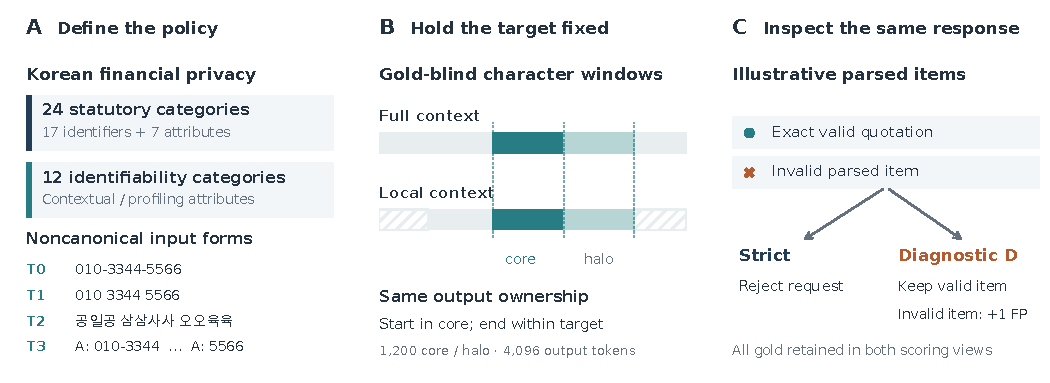
\includegraphics[width=\textwidth]{figures/benchmark-overview.pdf}
\caption{\textbf{From detection policy to an auditable extraction task.}
(A) The 36-category policy and illustrative T0--T3 forms of one synthetic
identifier. T2 reads zero one zero, three three four four, five five six six in Korean. (B) Full and local context share core ownership, a following
halo and the output budget; the schematic is not to scale. (C) An illustrative
normally completed response with one valid and one invalid parsed item:
strict scoring rejects the request, while D retains the valid item and
charges an invalid-item false positive. Both retain all gold. This example
explains the scoring contract, not a causal partition of model ability.}
\Description{Three panels connect the 24 statutory and 12 identifiability
categories, a matched full/local context window, and strict versus itemwise
validation of the same received response. Korean digit words and split turns
illustrate noncanonical synthetic identifier forms.}
\label{fig:overview}
\end{figure*}



Recognizing a well-formed identifier is only one part of detecting personal information in financial text. A customer may dictate an account number as \textup{일일공 에 일이삼 에 사오육칠팔구} (spoken digits for 110-123-456789, with \textup{에} marking separators), split it across turns, or provide a partially masked value. A repayment difficulty or an upcoming life event can also convey personal information without resembling an identifier. A benchmark for data loss prevention (DLP) must therefore make both the detection policy and the conditions of recognition explicit.

Korean finance brings these requirements together. Statutory categories include customer identifiers and financial attributes beyond conventional name--address--phone labels (\S\ref{sec:taxonomy}). Some additional attributes are useful to study because they can support profiling~\cite{staab2024beyond}, even when they are not separately enumerated in our statutory mapping. Treating all such targets as an undifferentiated PII label obscures what a detector covers; treating all detected spans as legally requiring redaction conflates evaluation policy with legal obligation.

Document context introduces a second ambiguity. Surrounding text may establish that an amount or statement concerns a person, but a long record may also contain unrelated details and multiple customers. Moreover, accepting a long input does not ensure that a model can enumerate all sensitive spans within a finite response. Full-document and chunked extraction are difficult to compare when they also change the amount of output requested. This motivates our central question: \emph{under an explicit Korean financial detection policy and a fixed output task, how does wider context affect typed-span recovery?}

Existing work studies query-aware PII protection~\cite{shen2025piibench}, multilingual detection~\cite{vats2026redact}, Korean dialogues~\cite{fei2024kdpii} and court judgments~\cite{hahm2025thunderdeid}. Korean financial benchmarks additionally establish the value of domain-specific evaluation~\cite{hwang2025twice,lee2025nmixx}. \kiii{} connects these directions through a shared taxonomy, controlled input variation and a matched context comparison. We contribute:
\begin{enumerate}
  \item \textbf{An auditable detection policy:} 36 categories separating statutory grounds (24) from additional identifiability concerns (12), with category definitions and masking metadata kept distinct (\S\ref{sec:taxonomy}).
  \item \textbf{A controlled financial testbed:} 1,440 synthetic documents and 218,664 spans covering ten document types, multiple subjects and T0--T3 variation, with code-generated identifiers and span-level provenance (\S\ref{sec:benchmark}).
  \item \textbf{A matched context evaluation:} 22 completed conditions from 12 LLMs provide ten within-model context pairs with identical target regions and output budgets; three frozen baselines provide document-level references (\S\ref{sec:setup}). Archived-response diagnostics distinguish response rejection, grounding errors and missed spans while preserving the primary exact score.
\end{enumerate}


\section{Related Work}
\label{sec:related}

\paragraph{PII detection and anonymization.}
PII-Bench~\cite{shen2025piibench} evaluates query-aware privacy protection, including multi-subject settings. REDACT~\cite{vats2026redact} organizes multilingual detection by sensitivity and disclosure form, while Mind the Gap~\cite{zafar2026mindthegap} examines distribution shifts. These works motivate evaluation beyond canonical entity recognition. \kiii{} focuses on Korean financial categories and input transformations under a shared operational policy. The Text Anonymization Benchmark~\cite{pilan2022tab} distinguishes direct and quasi-identifiers and evaluates disclosure risk. Anonymization systems~\cite{staab2025anonymizers,yang2025rupta} and re-identification benchmarks~\cite{krco2026ratbench} address privacy--utility trade-offs. Our task is narrower: exact recovery of typed spans, without claiming that extraction F1 measures residual disclosure risk or anonymization quality.

\paragraph{Korean PII.}
KDPII~\cite{fei2024kdpii} studies de-identification in Korean dialogues; Jang et al.~\cite{jang2024koreanpiiner} develop a Korean personal-information recognizer. Thunder-DeID~\cite{hahm2025thunderdeid} provides a detailed taxonomy for court judgments. These resources establish Korean PII detection as a distinct evaluation setting. We complement them with explicit financial category mappings, recorded surface-form operations and a fixed-output comparison of document context. This scope differs from conversational text anonymization~\cite{albanese2026anonymous} and from contextual privacy judgments about appropriate disclosure~\cite{mireshghallah2024confaide,shao2024privacylens}.

\paragraph{Korean financial language evaluation.}
TWICE~\cite{hwang2025twice} introduces KorFinMTEB for Korean financial embedding evaluation. NMIXX~\cite{lee2025nmixx} studies Korean--English financial embeddings and introduces KorFinSTS. KFinEval-Pilot~\cite{hwang2025kfineval} evaluates financial knowledge, legal reasoning and toxicity; KRX Bench~\cite{son2024krx} evaluates company knowledge across markets. \kiii{} extends this domain-specific evaluation agenda to privacy detection: recovering which text spans fall under an explicit policy, rather than measuring financial knowledge or semantic similarity.


\section{Taxonomy}
\label{sec:taxonomy}

%% ~0.6 page. Table 1 = compact category table. Full statute quotes → appendix / repo.
Our taxonomy has two tiers and two kinds. \textbf{Tier L (Legal)} groups 24 operational categories grounded in Korean statutes and regulations: the Personal Information Protection Act (PIPA) \S23--24 and Enforcement Decree \S18--19 (sensitive and unique identifying information); the Credit Information Act (CIA) \S2 and its Enforcement Decree \S2, which lists 성명·주소·전화번호 (name, address and telephone number), e-mail and SNS addresses, the four national identification numbers, \emph{CI/DI and customer-distinguishing identifiers specified in the Decree} (\S2\,③), and business/corporate registration numbers (\S2\,④); the Real Name Financial Transactions Act \S4 (transaction information); and the Electronic Financial Transactions Act \S2(10) (access media). \textbf{Tier I (Identifiability)} contains additional categories that act as quasi-identifiers~\cite{pilan2022tab} or, when aggregated, enable profiling and personalised social engineering; membership in Tier I is a benchmark design choice, not a claim that these categories lack legal protection.

Each category is an \textbf{identifier} (a name or value used to refer to a person, organization or account) or an \textbf{attribute}. CIA \S2(1)(a) defines identifying information as credit information \emph{only when combined with} transaction, creditworthiness or capacity information; we separately specify a benchmark policy: L-identifiers and sensitive information are \nolinkurl{must_mask}, other L-attributes are \nolinkurl{mask_if_linked}, and Tier I is \nolinkurl{detect_only}. These are operational metadata, not a finding that every occurrence legally requires redaction. Corporate identifiers are retained as financial-record targets, not asserted to identify natural persons. Table~\ref{tab:taxonomy} lists the 36 categories (17 L-identifier, 7 L-attribute, 12 I-attribute). Staff names are annotated as PII with a \nolinkurl{subject_role} of \emph{staff}; institution and product names, biometric templates and unattributed amounts are excluded.

\paragraph{A shared operational policy.}
All 36 categories are scored for every system. Prompted models receive their definitions; baseline labels use frozen mappings. L/I indicates the basis for inclusion, not a sensitivity ranking. Scores measure coverage of this operational policy, not a model's legal or cultural beliefs.

\begin{table}[t]
\caption{Taxonomy overview: all 36 categories, with abbreviated labels. L denotes Legal and I denotes Identifiability.}
\label{tab:taxonomy}
\small
\begin{tabularx}{\columnwidth}{@{}>{\RaggedRight\arraybackslash}p{0.23\columnwidth}>{\RaggedRight\arraybackslash}X@{}}
\toprule
\textbf{Tier / kind} & \textbf{Categories} \\
\midrule
L / identifier\newline (17) & name; RRN; foreigner reg.\ no.; passport; driver's licence; phone; address; e-mail; online handle; customer ID; business reg.\ no.; corporate reg.\ no.; bank account; securities account; card; contract no.; access credential. \\
\addlinespace
L / attribute\newline (7) & credit transaction; transaction record; delinquency; financial capacity; credit score; public record; sensitive information. \\
\addlinespace
I / attribute\newline (12) & DOB/age; gender; nationality; family relation; employer/position; education; life event; investment profile; consultation content; service usage; device/IP; location mention. \\
\bottomrule
\end{tabularx}
\par\smallskip
\begin{minipage}{\columnwidth}
\RaggedRight\small
\textit{Policies.} L identifiers and sensitive information: must mask.
Other L attributes: mask if linked. I attributes: detect only.
Full subtypes, statutory citations and format rules are in the taxonomy specification.
\end{minipage}
\end{table}


\section{Benchmark Construction}
\label{sec:benchmark}

\paragraph{Slot-filling generation.}
We separate identifier generation from document composition to obtain mechanically traceable span offsets. An LLM composes each document from a plan (document type, number of subjects, target length, variation level) using typed slots such as \texttt{\{\{bank\_account\_no:1\}\}} for identifiers and inline tags \texttt{[[credit\_transaction:1]]…[[/…]]} for attribute spans. Code then fills identifier slots with synthetic values, applying supported checksum rules and format templates, records character offsets and entity identity, and rejects documents flagged by its unslotted-identifier checks. Ten financial document types cover forms, transaction records, agreements, transcripts and reports.

\paragraph{Surface-form variation (Figure~\ref{fig:overview}).}
Each document is assigned a level: \textbf{T0} canonical, \textbf{T1} formatting (separator changes, regrouping, partial masking, affixes), \textbf{T2} lexical (Korean-numeral dictation \textup{공일공 삼삼사사} (spoken digits: 010 3344), including mixed Sino-Korean and native forms such as \textup{삼하나육사} (3164, using native Korean \textup{하나} for \emph{one}), Hanja/fullwidth digits, OCR confusables, STT digit errors, leftover spoken separators \textup{에}/\textup{다시} (\emph{e/dasi}, used as separator tokens)), and \textbf{T3} structural (a value split across turns, agent read-back, missing or wrong keyword anchors, coreference-only mentions, multi-subject interleaving, tables, negated/hypothetical mentions). Span metadata records applied operations and a design-based regex-catchability flag; the flag is not a measured detector outcome. T levels specify permitted operations rather than matched rewrites of the same documents, so comparisons across levels are stratified evaluations, not paired causal effects. Transcript numeral rendering uses 70\% Arabic, 20\% Hangul and 10\% mixed forms, with a 20\% pre-masked subset: design settings, not production frequencies. Intentional encoded evasion is outside this input distribution. The generator also injects annotated hard negatives, including order numbers, public hotlines, placeholders and unattributed amounts.

\paragraph{Corpus.}
The preview contains 1,440 documents and 218,664 spans: 144 documents per type, 360 per T level, and 480 per customer-subject count (1, 3 or 8). GLM-5.2-FP8 composed 820 accepted documents and GPT-6 Astra composed 620. Both are API generators; neither enters the headline detector ranking. Realized document lengths range from 1,168 to 43,576 Unicode characters (median 7,449); these are not model-tokenizer measurements. All documents form one evaluation set, named \texttt{test}; no training or validation split is provided.

\paragraph{Automatic validation.}
All 1,440 documents pass the release checks for schema, span offsets and surface text, category membership, applicable identifier constraints and generation-plan requirements. Exact duplicate document text is rejected. Attribute boundaries originate in composition tags and operational boundary rules; successful structural checks do not establish semantic completeness or production realism. We retain generator, operation and subject-role provenance for stratified audits.

\paragraph{Practitioner appropriateness review.}
Five reviewers with financial-sector employment experience each inspected a different 10\% sample; sample overlap and selection records are unavailable. They judged the documents broadly similar to financial-sector documents and suitable for use as a dataset. This qualitative review assessed document appropriateness, not span-label correctness or boundary agreement; no inter-annotator agreement statistic is claimed.

\paragraph{Task.}
The primary task is typed span extraction, scored by exact category-and-boundary micro-F1. The analysis reports operational coverage of the fixed policy, rather than anonymization quality, residual disclosure risk or semantic utility.



\section{Evaluation Protocol and Response Diagnostics}
\label{sec:protocol}

We distinguish response acceptance, item grounding and typed-span recovery.
They use different denominators: valid JSON may contain no PII, while a
rejected response may mix correct quotations with invalid items.

\subsection{A fixed output task under different context}
Let a document contain $n$ Unicode code points. For request $j$, define a
non-overlapping core $C_j=[s_j,e_j)$ of at most $c=1{,}200$ characters and a
target $T_j=[s_j,\min(n,e_j+h))$, with following halo $h=1{,}200$.
The full condition supplies the entire document as context. The local
condition supplies $[\max(0,s_j-h),\min(n,e_j+h))$. Both also supply the
same target string and core length, with the same category definitions and
output cap. Partitioning uses text length only; it does not inspect gold
categories, subject identities or span locations.

An output item specifies a category, an exact target quotation and a
one-based occurrence index, counting overlapping occurrences. Its span is
owned by the request containing its start in $C_j$; its end may extend into
the following halo but not beyond $T_j$. Ownership avoids duplicate mentions across requests; identical category--boundary
predictions are also deduplicated. Quotation and occurrence replace numeric
offset generation but still require correct source localization.

The output task is held fixed, not the input length or inference cost.
Mentions extending beyond their owner's target remain gold false negatives
if they cannot be represented. A boundary audit confirms that all 218,664 gold spans fit their owning
targets; none is excluded or made unrepresentable by these windows. The contrast measures additional context within this extraction interface.

\subsection{Primary strict extraction}
Strict evaluation requires normal completion, the specified JSON root and
item structure, known labels, exact quotation anchoring and valid ownership
for every item in a response. If any item fails, that request contributes
no predictions. Truncated, terminal-failure and unparseable responses are
also empty. Gold spans remain in every case. Micro-precision and recall use
corpus-aggregated exact typed-span counts, with
\begin{equation}
 F_1=\frac{2\mathrm{TP}}{2\mathrm{TP}+\mathrm{FP}+\mathrm{FN}}.
\end{equation}
This primary score measures end-to-end extraction under the frozen contract.
Atomic rejection can suppress both valid and invalid items in the same
response, so it should not be read as a direct count of all recognizable PII.

\subsection{Post-hoc diagnostic views}
We replay archived responses without another model call. The diagnostic
parser permits removal of a single whole-response JSON fence and validates
parsed items independently. It retains exactly anchored valid items and
charges one exact false positive for each invalid parsed item. Let $I$ be
this invalid-item count and $\mathrm{FP}_a$ the unmatched anchored predictions.
The detection proxy uses $\mathrm{FP}_D=\mathrm{FP}_a+I$ in precision and
F1; recall includes all gold, including gold belonging to failed requests.
Thus keeping valid siblings does not make malformed items disappear without
a penalty. We call these measures D-P, D-R and D-F1.

Structural compliance is measured separately over \emph{all requests}.
It requires normally completed raw JSON with the prescribed field types
and no duplicate keys; JSON fences fail this test. It does not require
that a category belongs to the taxonomy or that a quotation exists in the
target. The empty-list rate also uses all requests and is computed after
the diagnostic whole-response fence parsing. A well-formed empty list can
therefore increase compliance without recovering any sensitive text.

Grounding diagnostics classify parsed-item failures by schema, category,
quotation, occurrence and core ownership. Gold-oriented summaries further
distinguish exact hits, wrong labels at exact boundaries, partial overlaps
and unresolved misses. These priority categories describe observations;
they do not identify the cause of a model's error. An unanchorable item
cannot be treated as evidence that any particular gold mention was detected.

No view repairs spelling, boundaries or labels, searches fuzzily, consults
gold to reinterpret an output, or drops failed requests. Terminal and
unparseable responses contain no usable parsed-item count and remain empty;
we do not invent an item penalty for them. The diagnostic also preserves
the original JSON parser's last-value behavior for duplicate keys while
flagging them as noncompliant. It cannot recover overwritten values.
Consequently D-F1 is an observable detection proxy, not format-independent
latent ability, and neither D-F1 nor character overlap replaces the primary
strict score.

% Queue wide floats early so they appear beside results/error analysis,
% rather than after the conclusion among the references. Captions and data
% are unchanged; source declaration order controls the printed float order.
\begin{figure*}[!t]
\centering
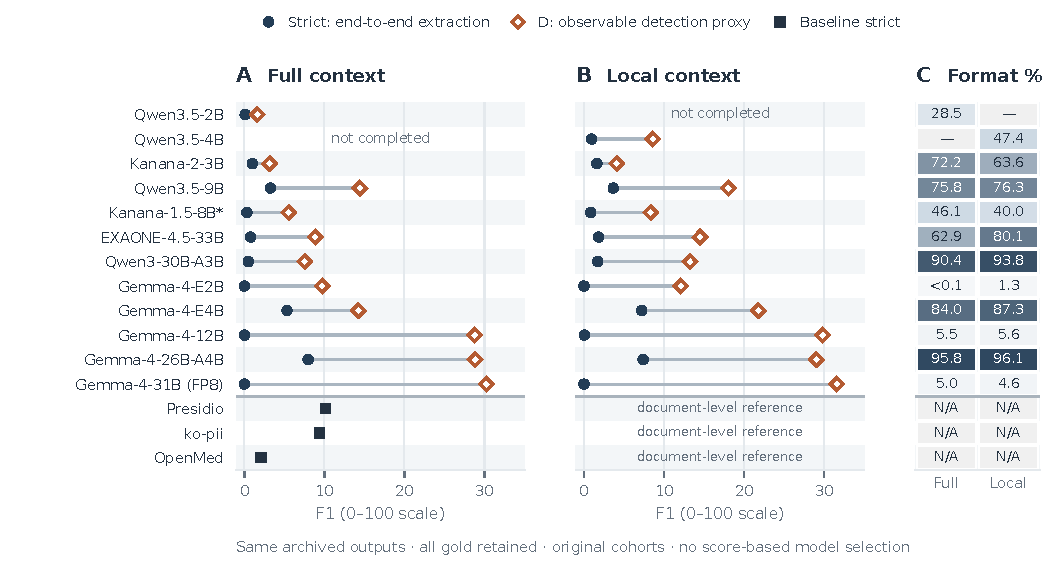
\includegraphics[width=\textwidth]{figures/score-portrait.pdf}
\caption{\textbf{Output validity and span recovery differ.}
Strict exact F1 (filled circles) and D-F1 (open diamonds) from the same archived
outputs, by full (A) and local (B) context. Connecting segments identify two
scoring views, not causal effects or confidence intervals. (C) Structural
compliance over all requests, which is not strict response acceptance.
Baseline squares are document-level strict references; D and format are N/A.
Missing conditions are explicitly marked. *Kanana-1.5-8B: 1,438 documents;
others: 1,440. All gold and invalid-item penalties remain in D. Execution
blocks differ; the display is descriptive, not a verified common-capacity ranking.}
\Description{Aligned full and local dot plots show all 22 completed LLM
conditions, with three document-level baseline references. Many Gemma runs
have near-zero strict F1 but higher diagnostic F1. Adjacent cells display
format compliance, including high compliance for Qwen3-30B and low compliance
for Gemma-12B and Gemma-31B. Missing Qwen pairs are not plotted as zeros.}
\label{fig:score-portrait}
\end{figure*}

\begin{figure*}[!t]
\centering
% Trim only the verified blank top/bottom PDF padding; preserve plot scale.
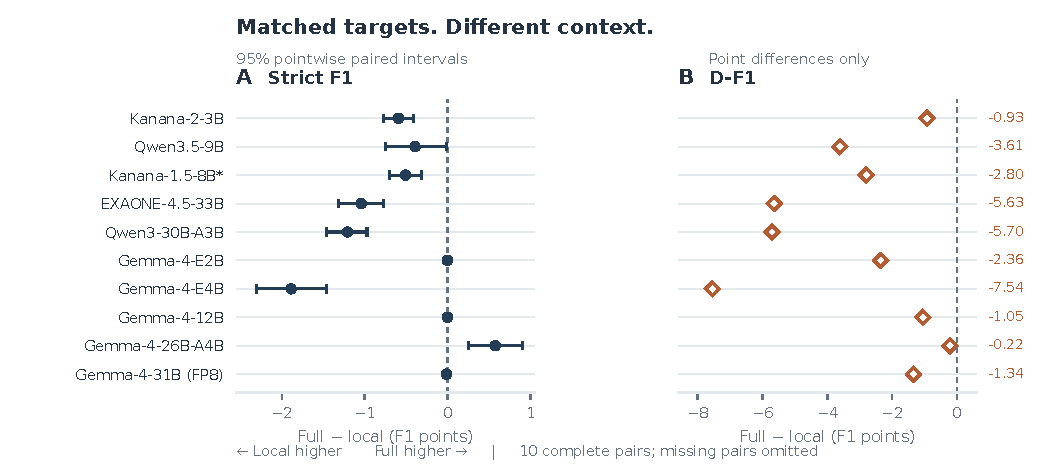
\includegraphics[trim=0 4bp 0 4bp,clip,width=\textwidth]{figures/context-contrasts.pdf}
\caption{Within-model full-minus-local contrasts on each model's original
cohort. Negative values favor local context. Left: strict F1 and pointwise
95\% document-paired bootstrap intervals (2,000 draws, seed 0). Right:
D-F1 point differences; no diagnostic confidence intervals are implied.
*Kanana-1.5-8B uses 1,438 documents; other pairs use 1,440. These are
post-hoc within-model comparisons, not an all-model common-capacity ranking.}
\Description{Two aligned panels show strict F1 differences with intervals
and diagnostic F1 point differences for ten models. Nine strict differences
and all ten diagnostic differences favor local context. Gemma-26B-A4B is
the strict exception. The intervals for Gemma-E2B and Gemma-12B cross zero.}
\label{fig:context-contrasts}
\end{figure*}

%% Generated from pinned ADR-0038 summary.csv; do not edit numbers.
\begin{table*}[t]
\caption{Completed-run strict scores and post-hoc diagnostics. Scores and rates use 0--100; invalid items are counts. Fmt: structural compliance; Empty: empty-list rate; D: observable detection proxy with invalid-item exact-FP penalties. F/L: full/local; Doc: document-level baseline. *Kanana-1.5-8B uses 1,438 documents; others use 1,440. Baseline diagnostics are not applicable.}
\label{tab:response-diagnostics}
\small
\begin{tabular*}{\textwidth}{@{\extracolsep{\fill}}llrrrrrrr@{}}
\toprule
System & Context & Strict F1 & Fmt & Empty & D-Prc & D-Rec & D-F1 & Invalid items \\
\midrule
Qwen3.5-2B & F & 0.12 & 28.48 & 1.38 & 3.39 & 1.08 & 1.64 & 64,498 \\
Qwen3.5-4B & L & 0.97 & 47.37 & 4.99 & 12.59 & 6.52 & 8.59 & 83,370 \\
Kanana-2-3B & F & 1.02 & 72.22 & 2.18 & 5.64 & 2.20 & 3.17 & 75,465 \\
Kanana-2-3B & L & 1.62 & 63.62 & 8.69 & 12.02 & 2.47 & 4.09 & 31,764 \\
Qwen3.5-9B & F & 3.27 & 75.79 & 16.83 & 18.58 & 11.81 & 14.44 & 96,349 \\
Qwen3.5-9B & L & 3.66 & 76.35 & 13.82 & 22.62 & 15.02 & 18.05 & 87,614 \\
Kanana-1.5-8B* & F & 0.33 & 46.09 & 0.74 & 5.11 & 6.09 & 5.55 & 235,147 \\
Kanana-1.5-8B* & L & 0.84 & 40.01 & 0.23 & 12.01 & 6.40 & 8.35 & 83,701 \\
EXAONE-4.5-33B & F & 0.81 & 62.88 & 26.36 & 8.67 & 9.07 & 8.87 & 186,354 \\
EXAONE-4.5-33B & L & 1.85 & 80.13 & 29.86 & 14.68 & 14.33 & 14.50 & 145,380 \\
Qwen3-30B-A3B & F & 0.52 & 90.42 & 53.06 & 9.38 & 6.31 & 7.55 & 123,733 \\
Qwen3-30B-A3B & L & 1.73 & 93.78 & 17.61 & 15.04 & 11.84 & 13.25 & 123,434 \\
Gemma-4-E2B & F & $<0.01$ & 0.04 & 46.69 & 16.55 & 6.89 & 9.73 & 62,457 \\
Gemma-4-E2B & L & $<0.01$ & 1.28 & 54.11 & 28.10 & 7.70 & 12.09 & 28,868 \\
Gemma-4-E4B & F & 5.34 & 84.00 & 5.62 & 16.35 & 12.64 & 14.25 & 129,082 \\
Gemma-4-E4B & L & 7.23 & 87.34 & 8.88 & 30.42 & 16.98 & 21.79 & 65,661 \\
Gemma-4-12B & F & 0.04 & 5.55 & 12.19 & 31.94 & 26.15 & 28.76 & 85,401 \\
Gemma-4-12B & L & 0.05 & 5.55 & 7.79 & 30.84 & 28.85 & 29.81 & 92,237 \\
Gemma-4-26B-A4B & F & 7.97 & 95.77 & 12.29 & 34.78 & 24.60 & 28.82 & 69,113 \\
Gemma-4-26B-A4B & L & 7.40 & 96.10 & 7.19 & 31.14 & 27.20 & 29.04 & 84,943 \\
Gemma-4-31B (FP8) & F & $<0.01$ & 4.98 & 5.74 & 29.00 & 31.59 & 30.24 & 102,275 \\
Gemma-4-31B (FP8) & L & 0.02 & 4.56 & 4.17 & 28.86 & 34.86 & 31.58 & 104,568 \\
\midrule
Presidio & Doc & 10.15 & -- & -- & -- & -- & -- & -- \\
ko-pii & Doc & 9.43 & -- & -- & -- & -- & -- & -- \\
OpenMed & Doc & 2.09 & -- & -- & -- & -- & -- & -- \\
\bottomrule
\end{tabular*}
\end{table*}


\begin{figure*}[!t]
\centering
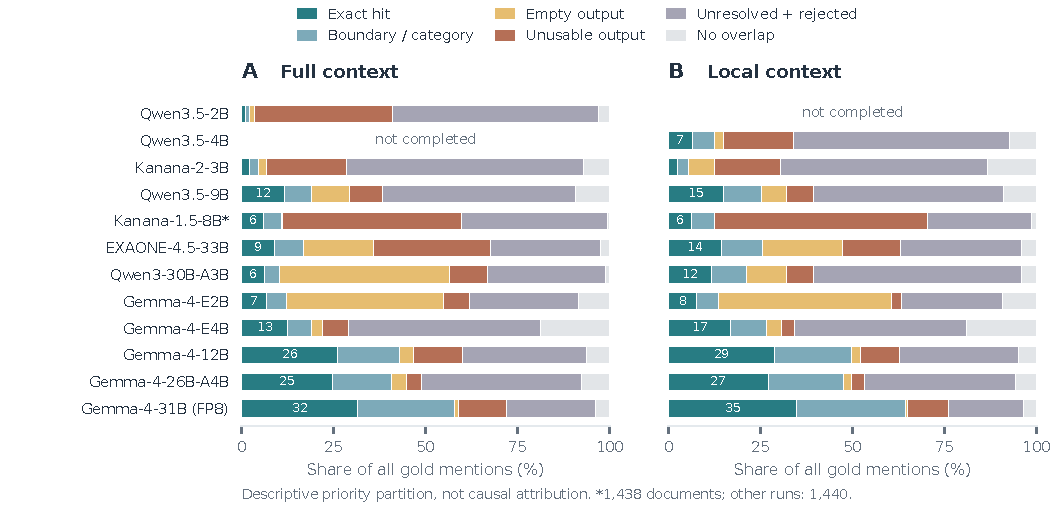
\includegraphics[width=\textwidth]{figures/error-atlas.pdf}
\caption{\textbf{Similar low scores conceal different observable failures.}
All-gold priority partitions for 22 completed LLM conditions. Exact-hit shares
are D-recall; integers inside teal bars are rounded percentages. Boundary/category
mismatches have anchored overlap but fail exact typed matching. Unresolved
misses with rejected items do not establish detection. Unusable output comprises
terminal/truncated responses and JSON/root failures; empty output is separate.
Segments are descriptive, not causal contributions to F1. Missing conditions
are not zero. *Kanana-1.5-8B: 218,197 gold mentions; others: 218,664.}
\Description{Paired horizontal stacked bars account for every gold mention.
Qwen3-30B full is dominated by empty-output misses, Kanana-8B by unusable
outputs, and Gemma-31B local has larger exact-hit and boundary/category
overlap portions while retaining a substantial unresolved remainder.}
\label{fig:error-atlas}
\end{figure*}

\section{Experimental Setup}
\label{sec:setup}

\paragraph{Systems and scope.}
We report 22 completed conditions from 12 language models and three frozen baselines (Figure~\ref{fig:score-portrait}). The initial Qwen3.5-2B/4B and Kanana-2-3B runs were extended after formatting failures were observed; the extension is exploratory. Only Qwen-2B full and Qwen-4B local have complete artifacts, so their opposite conditions are omitted. No model is trained on the benchmark; GLM/Astra are generators only. All runs use 1,440 documents except Kanana-1.5-8B, whose recorded length exclusions leave 1,438. Original cohorts and failed requests are retained.

\paragraph{Matched extraction target.}
All completed LLM conditions use the protocol in \S\ref{sec:protocol}: 1,200-character cores and halos, with 4,096 output tokens. Baselines process documents using their frozen rules or token-classification windows; they are document-level references, not full/local pairs. No comparison treats the baseline interface as identical to the LLM extraction contract.

\paragraph{Baseline coverage.}
Our Presidio configuration uses direct Korean rule recognizers and custom account/card patterns; ko-pii uses fixed regex matches. OpenMed uses token-level argmax BIOES decoding and fixed fragment mappings. The frozen maps can emit 9, 17 and 13 of the 36 target categories, respectively. All 36 categories remain in the gold denominator: these baselines measure deployed configuration coverage, not equal-label recognition ability.

\paragraph{Execution and audit.}
Qwen/Kanana/EXAONE used BF16 vLLM serving; Gemma used BF16 except 31B (FP8 weights and KV cache). Recorded decoding and server settings differ across execution blocks (\S\ref{app:diagnostics}); cross-family results are descriptive, not a controlled scaling study. Gemma used an external runner. We reconstruct requests and replay every strict score and failure from archived responses, preserving the original execution metadata. Native count files were not supplied for independent capacity verification, and representative separate-pilot calibration is not established by the artifacts. We therefore do not claim a verified all-model capacity gate. Paired contrasts check matching data, protocol, model revisions, settings and recorded gates within each model. Pointwise 95\% intervals use 2,000 document-paired bootstrap samples (seed 0); analysis is post-hoc.

\paragraph{Implementation assistance.}
Claude and OpenAI Codex assisted implementation of generation, evaluation and analysis code and preparation of plotting code. Reported scores are computed from archived predictions by deterministic scoring and replay; generative models do not assign these scores. Dataset composition models and their use are specified in \S\ref{sec:benchmark}.


\section{Results and Analysis}
\label{sec:results}

The descriptive comparison (Figure~\ref{fig:score-portrait}) reports completed extraction systems, with strict scores kept separate from a detection diagnostic. Full breakdowns and paired intervals appear in \S\ref{app:result-layout}. Figure~\ref{fig:context-contrasts} visualizes the ten completed within-model comparisons.



\paragraph{Strict rejection can hide valid items.}
Presidio reaches 10.15 strict F1; the highest LLM strict score is 7.97 (Gemma-26B-A4B, full). For LLMs, strict scoring enforces the frozen response contract: one invalid item can suppress valid siblings. The itemwise replay in \S\ref{sec:protocol} retains valid anchored items while preserving invalid-item penalties and all gold. Its contrast with strict F1 describes usable evidence in the received output, not performance under an improved decoder.

Gemma-12B local moves from 0.05 strict F1 to 29.81 D-F1; Gemma-31B FP8 local reaches 31.58 D-F1 (28.86 precision, 34.86 recall). Format compliance alone is also insufficient: Qwen3-30B full has 90.42\% structurally compliant responses but only 7.55 D-F1, and 53.06\% of all requests return an empty list. Thus output acceptance, grounding and missed PII need separate denominators, not a success-only score.

\paragraph{Wider context does not ensure recovery.}
Local context has higher D-F1 in all ten completed pairs and higher strict F1 in nine. Strict full-minus-local differences range from $-1.89$ points (Gemma-E4B) to $+0.57$ (Gemma-26B-A4B); the latter reverses to $-0.22$ under D. The contrast measures extraction under this fixed output protocol, not an intrinsic inability to use long context. Cohort, decoding and generation differences preclude causal model-size conclusions. Strict recovery concentrates on identifiers: Gemma-26B-A4B full scores 15.99 F1 on L-identifiers but 0.49 on L-attributes and 0.23 on I-attributes. Presidio scores 20.12 on identifiers and zero on both attribute groups. This exposes limited policy coverage; missed categories alone do not establish legal or cultural beliefs.




\section{Error Analysis}
\label{app:diagnostics}
\label{app:result-layout}

Table~\ref{tab:response-diagnostics} keeps strict extraction, structural
compliance and detection on their respective denominators. Each full
1,440-document LLM run has 13,723 requests and 218,664 gold mentions;
Kanana-1.5-8B has 13,653 requests and 218,197 mentions over 1,438 documents.
No missing condition is imputed. Baseline format and D scores are N/A.



\subsection{Where unrecovered gold appears}
Figure~\ref{fig:error-atlas} partitions every gold mention using a fixed
priority: exact diagnostic hit; an owning request with unusable output or
an empty list; an anchored boundary/category mismatch; and otherwise an
unresolved miss with rejected items, or no overlapping prediction.
Unusable output includes terminal failure, truncation and invalid JSON/root
schema. Each row sums to its original gold count. These are descriptive
buckets: an unresolved rejected quotation does not establish detection of
any particular gold span, and priority assignment does not isolate causes.



\paragraph{Well-formed silence versus unusable output.}
Qwen3-30B full returns empty lists on 53.06\% of requests; those requests
own 100,873 gold mentions (46.13\% of all gold). In local context this
share falls to 10.83\%. This distinguishes abstention-like output from
JSON failure without claiming why the model omitted PII. Kanana-1.5-8B
local instead places 119,200 of 218,197 mentions (54.63\%) in requests
with invalid JSON. A single ``format failure'' rate would obscure both
the empty-output burden and its different gold coverage.

\paragraph{Source grounding includes output ownership.}
Among Gemma-31B local's 104,568 invalid parsed items, 98,200 (93.91\%)
quote target text but start outside the owning core; Gemma-26B-A4B local
has 76,806 such items out of 84,943 (90.42\%). These are not quotations
absent from the source. In a replay-verified Gemma-26B case, a returned
address begins 236 characters after the core ends. It exists in the
following halo, where a span may end but may not start. The result exposes
a burden of this extraction interface, not solely a failure to recognize
sensitive text. Invalid items still incur false positives under D, and
unresolved gold still incurs false negatives.

\paragraph{Recognition does not settle labels or boundaries.}
Gemma-31B local exactly recovers 34.86\% of gold; another 23.33\% has
same-category overlap with different boundaries. Exact-boundary wrong
labels account for 0.65\%, and other wrong-category overlaps for 5.63\%.
In one synthetic consultation case, the model reproduces the entire gold
clause but adds its final period. This is an exact-match error with
substantial textual overlap. Conversely, Qwen-9B local quotes the exact
contract identifier \texttt{2026-277485} but labels it as a customer ID.
These observations motivate reporting overlap and typed exact scores
together; neither proves semantic correctness or remaining disclosure risk.

\paragraph{Wrappers can hide valid evidence.}
A whole-response JSON fence is parseable in 89.66\% of Gemma-31B local
requests, despite its 0.017 strict F1. A selected fenced response contains
an exactly typed bank account and no invalid items: strict rejects the
response while D retains the account. The total strict--D gap cannot be
attributed to fences alone because itemwise acceptance and false-positive
accounting also change. The five archived illustrations use the minimum
SHA-256 request ID within specified model/error strata, followed by
lexicographic item/span selection. We verified source and response hashes,
reconstructed requests and replayed their outcomes. This purposive audit
illustrates failure definitions; it is not representative human annotation.

\paragraph{Serving provenance.}
Operator records report vLLM 0.30.0 for Qwen/Kanana/EXAONE (BF16,
temperature 1, top-$p$ 1), and vLLM 0.19.0 for Gemma, except 12B (0.30.0), on one H100 80GB
(temperature 1, top-$p$ 0.95, top-$k$ 64; thinking disabled).
Gemma-31B uses FP8 weights and KV cache; the others use BF16.
Runner and server inventories are distinct. Archived revisions, request/raw
hashes and original versus replay-source hashes preserve provenance;
replay does not establish deployment equivalence or native capacity.

\section{Discussion}
\label{sec:discussion}

\paragraph{Evaluate the policy and interface together.}
Strict F1 measures the complete extraction contract; D exposes valid
evidence in the same outputs. Their gap does not additively measure loss
caused by formatting. Identifier-heavy recovery leaves attribute coverage
unresolved. Character overlap cannot charge character false positives for
unanchorable items and must accompany invalid-item counts and exact
penalized precision. None of these measures certifies legal compliance.

\paragraph{Context benefits depend on the output task.}
All ten completed pairs favor local context on D-F1, but both conditions
already expose the same explicit target. The result does not show that
distant evidence is unnecessary. Attention dilution, instruction following
and output allocation are possible explanations, not established mechanisms.
Paired intervals describe document-resampling variation over this synthetic
collection and one execution per condition, not stochastic rerun or
production uncertainty. Shared generation plans may induce dependence;
semantic near-duplicate clusters remain unaudited. T levels use different
documents, not paired rewrites. Constrained generation, revised ownership
or punctuation-tolerant matching would define a new prospective experiment;
we do not retrofit them to improve scores on this test set.


\section{Conclusion and Limitations}
\label{sec:conclusion}

\kiii{} links a traceable Korean financial detection policy to noncanonical inputs and a matched context task. Across completed runs, output-contract failures obscure recoverable PII, while local context yields higher D-F1 in all ten completed pairs under this fixed interface. Reporting strict extraction, structural compliance and all-gold detection together exposes different failure modes without forgiving missed sensitive information.

\paragraph{Limitations and ethics.}
Synthetic documents and practitioner appropriateness review do not establish production representativeness or span correctness. Attribute boundaries may be ambiguous, and semantic near-duplicates have not been audited. T levels are not paired counterfactuals; STT frequencies are design settings. Post-hoc model extensions, decoding/precision differences, unavailable native counts and unverified pilot calibration limit generalization. The diagnostic is an observable proxy, not format-independent ability or legal compliance. No real customer records were used, though coincidental identifier matches remain possible. The preview is CC BY-NC 4.0; a formal release will follow.

\paragraph{Data availability.}
The dataset preview is available at \url{https://huggingface.co/datasets/nmixx-fin/kiii-kiii} (CC BY-NC 4.0). The dataset revision and completed-run scope reported here remain fixed.

\section*{Acknowledgment}
Claude and OpenAI Codex assisted manuscript drafting, restructuring and language revision. The authors retain responsibility for the claims, citations and final manuscript.


Kanana model attribution: Powered by Kanana.


\bibliographystyle{ACM-Reference-Format}
\bibliography{references}



\end{document}
